\subsection{Use Case Diagram}
The Use Case Diagram visually describes the behavioral capabilities of the Digital Farmer Assistance System from the perspective of its primary actors. This diagram ensures that all high-level functional requirements defined in the SRS are adequately accounted for by corresponding system interactions.

\begin{figure}[!htbp]
    \centering
    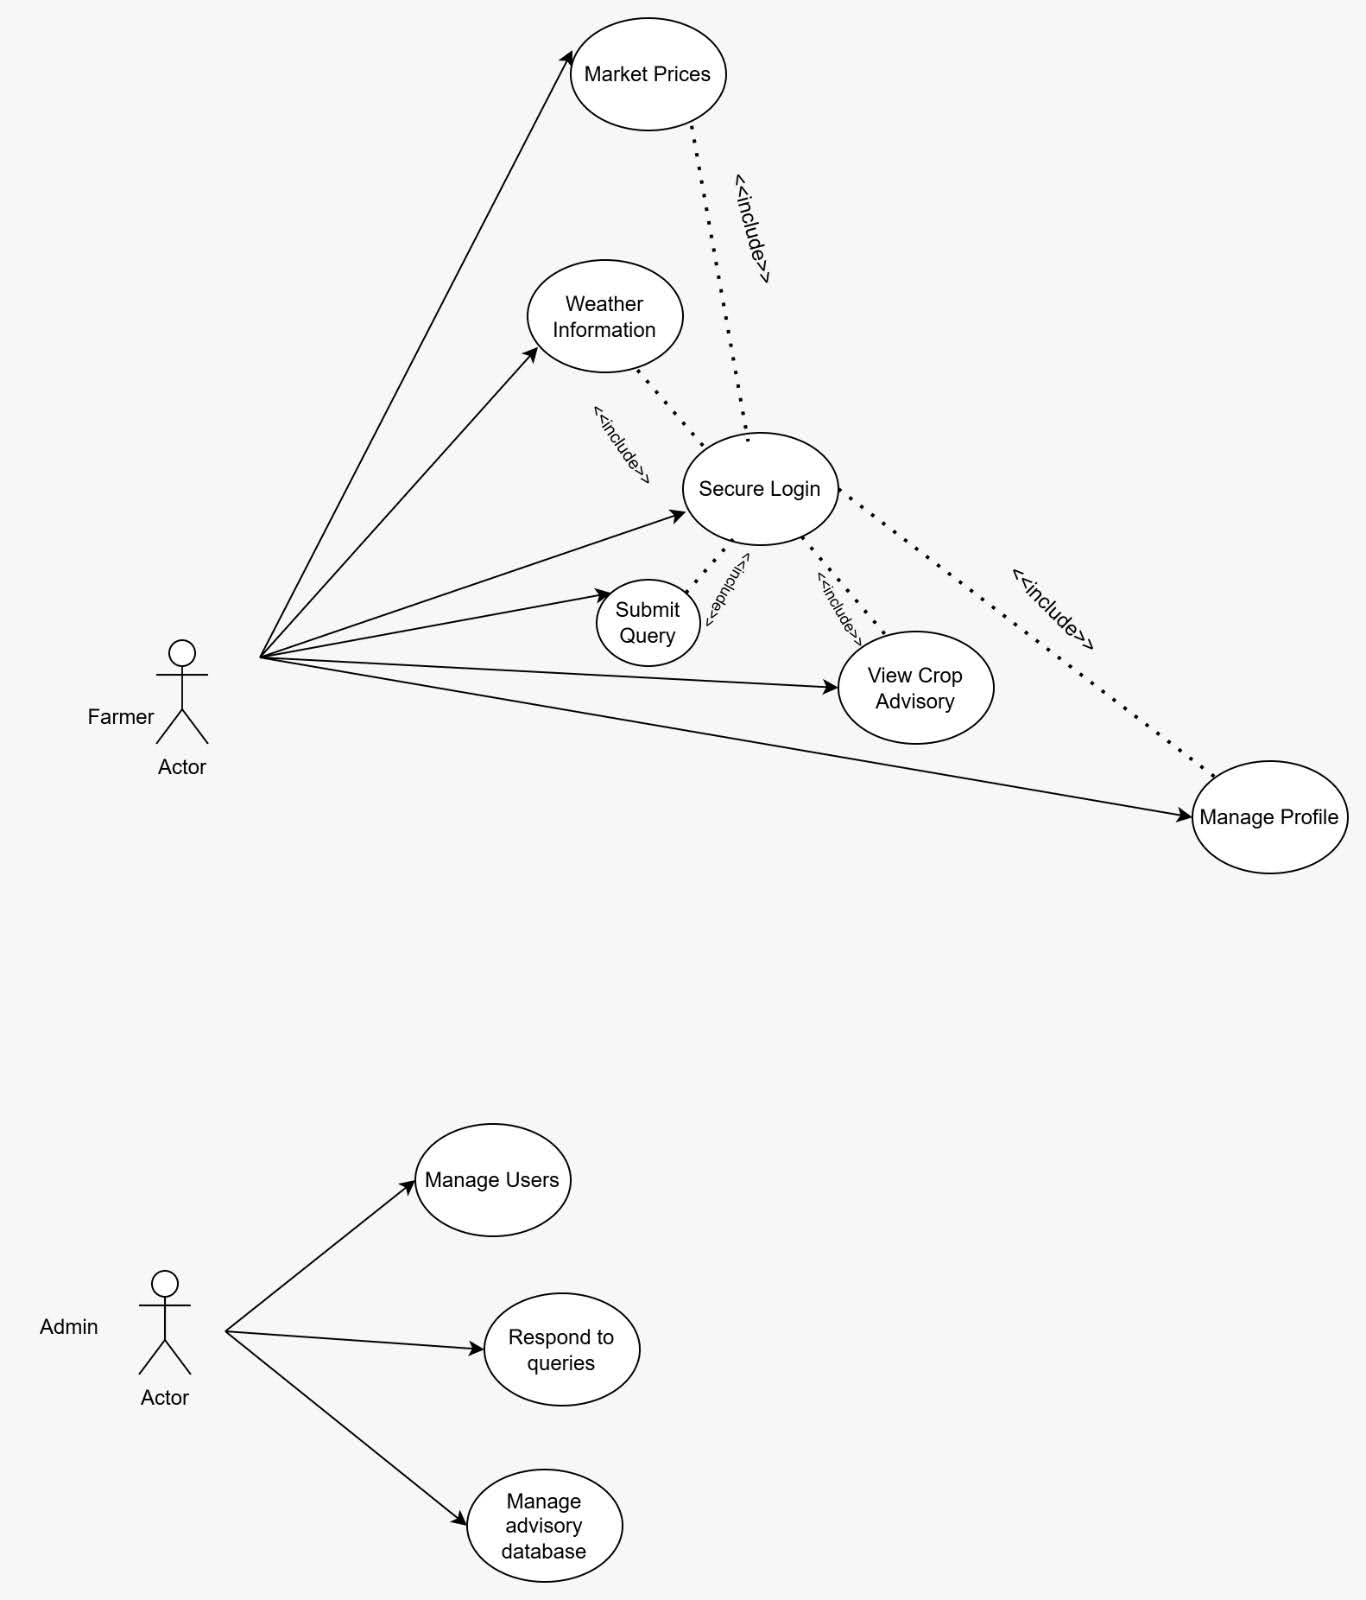
\includegraphics[width=0.85\textwidth]{../images/usecase.jpg}
    \caption{System Use Case Diagram}
    \label{fig:usecase}
\end{figure}

\textbf{Actors:}
\begin{itemize}
    \item \textbf{Farmer:} The primary end-user who consumes data and submits queries.
    \item \textbf{Admin (and Superadmin):} Personnel responsible for data entry, system modifications, user management, and expert query responses.
\end{itemize}

\textbf{Primary Use Cases:}
\begin{enumerate}
    \item \textbf{Farmer Interactions:}
    \begin{itemize}
        \item \textit{View Market Prices:} The farmer accesses a centralized dashboard displaying the latest commodity pricing (\textless\textless include\textgreater\textgreater\ Secure Login).
        \item \textit{View Weather Information:} The farmer accesses five-day forecast data localized to their defined region (\textless\textless include\textgreater\textgreater\ Secure Login).
        \item \textit{View Crop Advisory:} The farmer receives personalized data based on pre-registered crop types (\textless\textless include\textgreater\textgreater\ Secure Login).
        \item \textit{Submit Query:} The farmer transmits textual questions directly to agricultural experts (\textless\textless include\textgreater\textgreater\ Secure Login).
        \item \textit{Manage Profile:} The Farmer configures phone numbers, language preferences, and crop portfolios (\textless\textless include\textgreater\textgreater\ Secure Login).
    \end{itemize}
    
    \item \textbf{Admin Interactions:}
    \begin{itemize}
        \item \textit{Manage Users:} Reviewing farmer registrations and editing permission structures.
        \item \textit{Respond to Queries:} Administrating expert answers to farmer-submitted inquiries.
        \item \textit{Manage Advisory Database:} Performing CRUD operations on crop knowledge base articles.
        \item \textit{Manage Market Prices:} Entering newly verified commodity pricing metrics natively into the database.
        \item \textit{Manage Weather Data:} Establishing manual weather overrides inside the database fallback system.
    \end{itemize}
\end{enumerate}

\subsection{Class Diagram}
The Class Diagram delineates the structural framework of the software, explicitly defining system objects, their attributes, behavioral methods, and their inter-relationships, thereby bridging the conceptual design into actionable object-oriented engineering strategies.

\begin{figure}[!htbp]
    \centering
    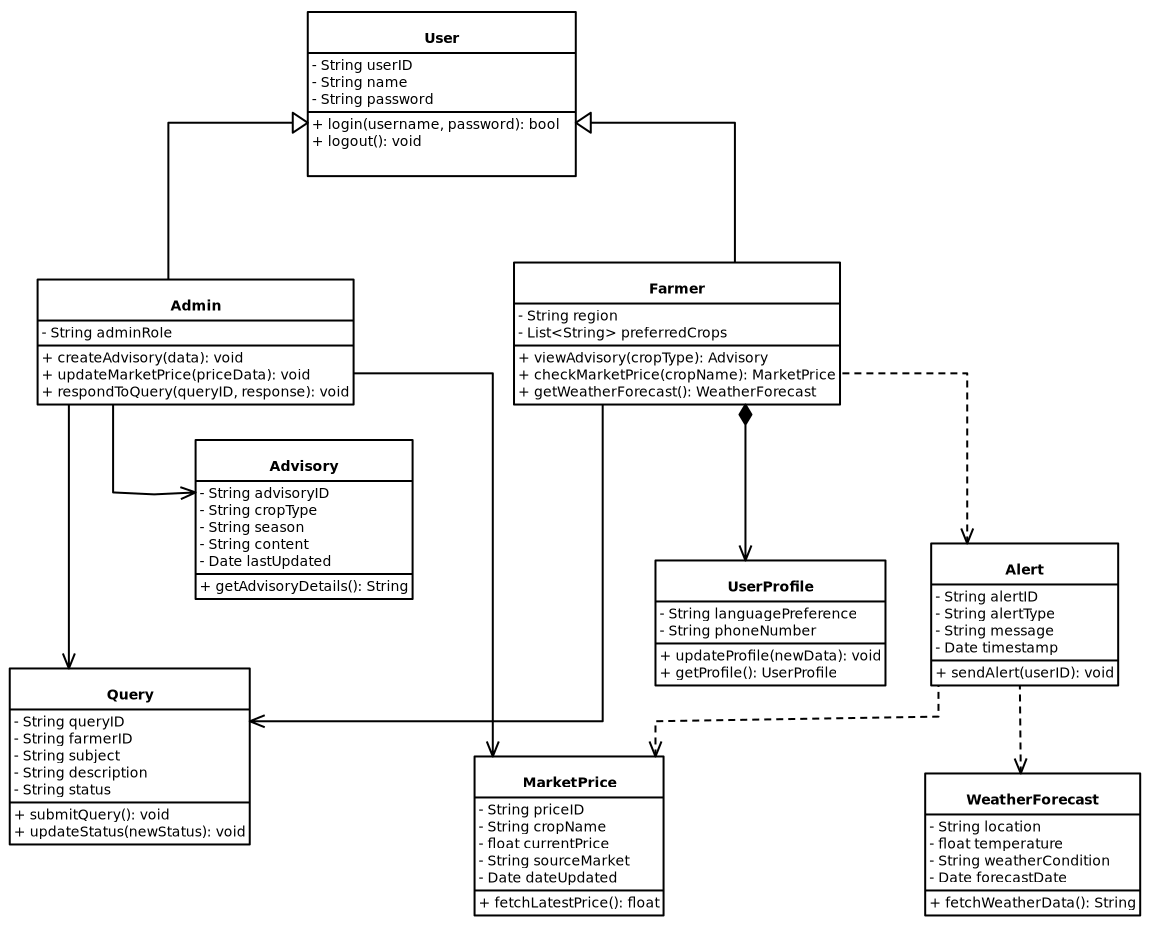
\includegraphics[width=0.85\textwidth]{../images/classdiagram.png}
    \caption{System Class Diagram}
    \label{fig:classdiagram}
\end{figure}

\textbf{Core Class Definitions:}
\begin{itemize}
    \item \texttt{User} (Abstract Base Class): Centralizes common authentication attributes (\texttt{userID}, \texttt{name}, \texttt{passwordHash}) and core methods (\texttt{login()}, \texttt{logout()}).
    \item \texttt{Admin}: Inherits \texttt{User}. Attributes include \texttt{adminRole}. Methods encompass authoritative interactions: \texttt{createAdvisory()}, \texttt{updateMarketPrice()}, and \texttt{respondToQuery()}.
    \item \texttt{Farmer}: Inherits \texttt{User}. Extends base class with \texttt{region} and \texttt{preferredCrops}. Specialized methodologies comprise \texttt{viewAdvisory()}, \texttt{checkMarketPrice()}, and \texttt{getWeather\-Forecast()}.
    \item \texttt{UserProfile}: Managed via composition by the \texttt{Farmer} class. Contains specific metadata including \texttt{language\-Preference} and \texttt{phone\-Number}, manipulatable via \texttt{update\-Profile()}.
    \item \texttt{Advisory}: Encapsulates structural data: \texttt{advisoryID}, \texttt{cropType}, \texttt{season}, \texttt{content}. Accessible via \texttt{getAdvisoryDetails()}.
    \item \texttt{Query}: Represents the interaction state: \texttt{queryID}, \texttt{subject}, \texttt{status}, and \texttt{response}, handled via \texttt{submitQuery()} and \texttt{updateStatus()}.
    \item \texttt{MarketPrice} \& \texttt{WeatherForecast}: Abstraction layers handling external data synchronization, tracking \texttt{sourceMarket}, \texttt{currentPrice}, \texttt{temperature}, and \texttt{weatherCondition}.
\end{itemize}

\textbf{Strategic Relationships:}
The software strictly employs hierarchical \textit{inheritance} for shared user functionality (Farmer/Admin $\leftarrow$ User). It mandates strong \textit{composition} mapping between the Farmer and their UserProfile (Farmer $\diamond\rightarrow$ UserProfile). Looser \textit{dependency} and \textit{association} relationships govern the dynamic interactions between the Farmer modules and rapidly volatile external data objects (Farmer $-\!-\!>$ MarketPrice).
